\section{Zielsetzung}
\label{sec:Zielsetzung}

In diesem Versuch soll die Verdampfungswärme von destilliertem Wasser ermittelt werden.
Dafür wird das destillierte Wasser erhitzt und die Temperaturabhängigkeit des Dampfdruckes gemessen, 
aus der resultierenden Dampfdruckkurve kann anschließend die gesuchte Verdampfungswärme berechnet werden.

\section{Theorie}
\label{sec:Theorie}

\begin{figure}
    \centering
    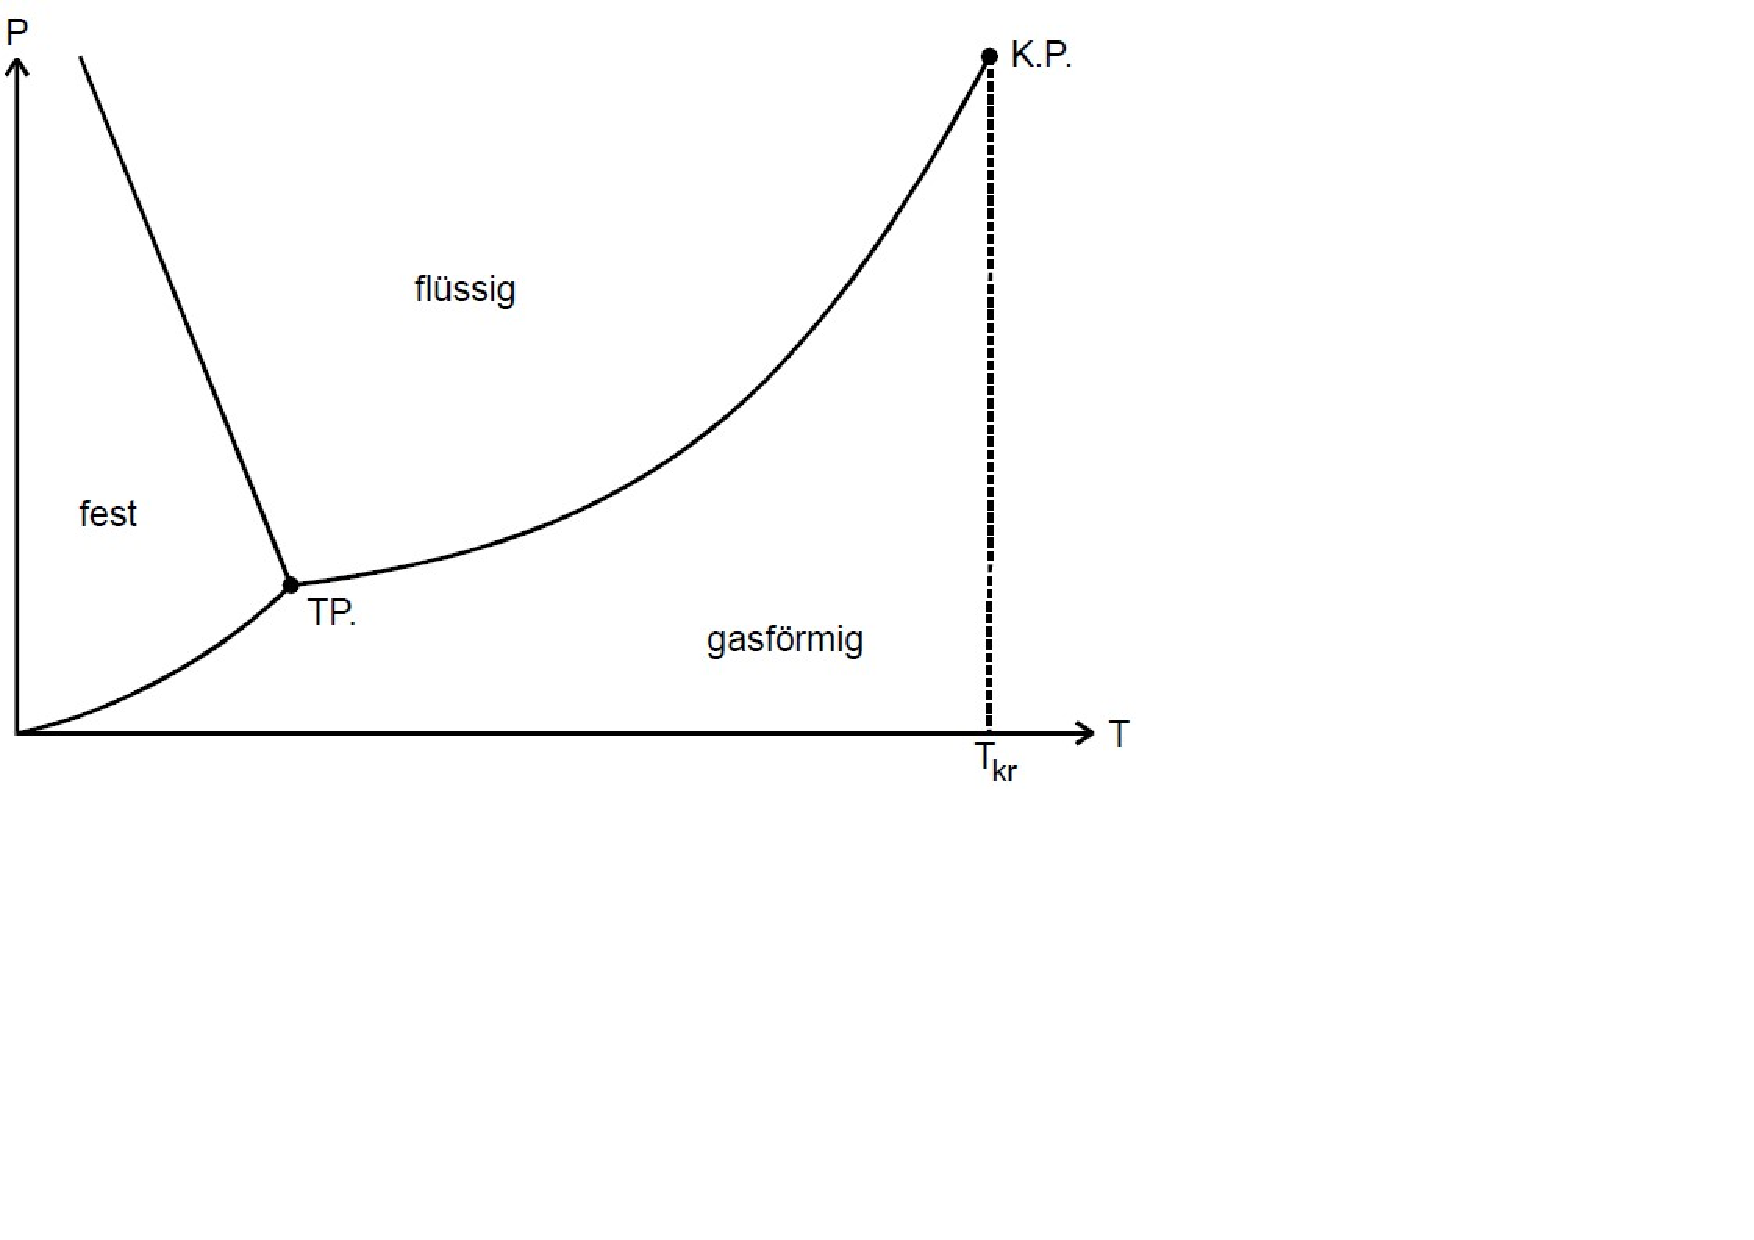
\includegraphics[height=7cm]{content/Bilder/Zustandsdiagramm.pdf}
    \caption{Qualitatives Zustandsdiagramm von Wasser. \cite{v203}}
    \label{fig:Zustandsdiagramm}
\end{figure}

\begin{equation}
    (V_{\symup{D}}-V_{\symup{F}})\symup{dp}=\frac{L}{T}\symup{dT}
    \label{eq:Clausius-Clapeyronsche Gleichung}
\end{equation}

\begin{equation}
    p(T)=p_0e^{-\frac{L}{R}\cdot\frac{1}{T}}
    \label{eq:Druck}
\end{equation}